\usepackage{color}
\usepackage{animate}
\usepackage{verbatim}

\usetheme{Warsaw}
\usecolortheme{whale}
\title{Introduction to \LaTeX}
\author{Shawn Tan}
\AtBeginSection[]
{
\begin{frame}{Table of Contents}
\tableofcontents[currentsection]
\end{frame}
}
\begin{document}
\maketitle
\begin{frame}
	\frametitle{Pronounciation}
	\begin{center}	 
	\huge \{lay,lah\}-teck
	\end{center}
\end{frame}
\begin{frame}
	\begin{center}
		\huge Samples
	\end{center}
\end{frame}
\begin{frame}
	\frametitle{A brief history}
	\begin{description}
		\item[1974] Donald Knuth stops submitting papers to American Mathematical Society(AMS)
		\item[1977] Knuth begins research into typography
		\item[1978] Knuth delivers an AMS Gibbs Lecture entitled Mathematical Typography
		\item[1979] \TeX finished\footnote{http://www.xent.com/FoRK-archive/feb98/0307.html}
		\item[Early 1980s] \LaTeX, a set of macros to make life easier when working with \TeX completed by Leslie Lamport. 
	\end{description}
\end{frame}
\begin{frame}
	\frametitle{Real programmers code with butterflies!}
	``When I wrote TeX originally in 1977 and ’78, of course I didn’t have literate programming but I did have structured programming. I wrote it in a big notebook in longhand, in pencil."- Knuth \footnote{Coders at Work}
\end{frame}
\begin{frame}
	\frametitle{Knuth's bank}
``Intelligence: Finding an error in a Knuth text.\\
~~~Stupidity: Cashing that \$2.56 check you got." \\- a Slashdot signature\footnote{http://www.stgray.com/quotes/programmingquotes.html}

\begin{center}
	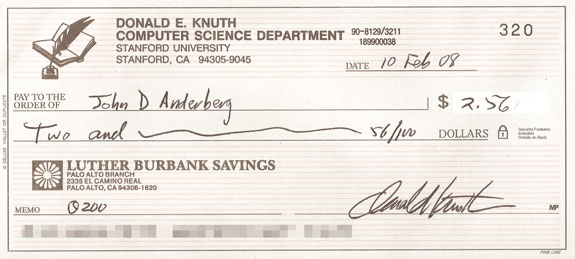
\includegraphics[scale=0.4]{hexadollar.jpg}
\end{center}

\end{frame}
\begin{frame}[allowframebreaks]
	\frametitle{\LaTeX - the (few) good parts}
	\huge
	\[e^{i\pi} + 1 = 0\]
	\framebreak
\[P(A|B) = \frac{P(B|A)P(A)}{P(B)}\]
\framebreak
\[
	P(x) = \frac{1}{{\sigma \sqrt {2\pi } }}e^{\frac{(x-\mu)^2}{2\sigma^2}}
\]
\framebreak
\[
	\frac{1}{\displaystyle 1+  \frac{1}{\displaystyle 1+ \frac{1}{\displaystyle 1+ \frac{1}{\pi}}}}
\]
\framebreak
\begin{center}
	Bibliography
\end{center}
\end{frame}
\begin{frame}
	\frametitle{\LaTeX - urghhh..}
	\begin{center}
		\huge
		Verbose, too much like programming
	\end{center}
\end{frame}

\begin{frame}[fragile]
	\frametitle{Line noise}

	\begin{verbatim}
	\[ M[i,j] = 
		\left\{ \begin{array}{l l} 0 & \quad \text{if } i=0 
		\text{ or } j=0\\
		M[i-1,j] & \quad \text{if } w_i > j\\
		\max \left( M[i-1,j-w_i] + v_i, M[i-1,j] \right)
		& \quad \text{if } w_i \leq j\\
\end{array} \right. \]

	\end{verbatim}
	\[ M[i,j] = \left\{ \begin{array}{l l} 0 & \quad \text{if } i=0 \text{ or } j=0\\ M[i-1,j] & \quad \text{if } w_i > j\\ \max \left( M[i-1,j-w_i] + v_i, M[i-1,j] \right)& \quad \text{if } w_i \leq j\\ \end{array} \right. \]
\end{frame}

\end{document}
